%
% File winlp2019.tex is modified based on File coling2018.tex
% 
% Contact: winlp-chairs@googlegroups.com
% if they can't help, contact: zhu2048@gmail.com & liuzy@tsinghua.edu.cn
%% Based on the style files for COLING-2018, which were in turn,
%% Based on the style files for COLING-2016, which were, in turn,
%% Based on the style files for COLING-2014, which were, in turn,
%% Based on the style files for ACL-2014, which were, in turn,
%% Based on the style files for ACL-2013, which were, in turn,
%% Based on the style files for ACL-2012, which were, in turn,
%% based on the style files for ACL-2011, which were, in turn, 
%% based on the style files for ACL-2010, which were, in turn, 
%% based on the style files for ACL-IJCNLP-2009, which were, in turn,
%% based on the style files for EACL-2009 and IJCNLP-2008...

%% Based on the style files for EACL 2006 by 
%%e.agirre@ehu.es or Sergi.Balari@uab.es
%% and that of ACL 08 by Joakim Nivre and Noah Smith

\documentclass[11pt]{article}
\usepackage{coling2018}
\usepackage{haldefs}
\usepackage{times}
\usepackage{url}
\usepackage{latexsym}
\usepackage{graphicx}
\usepackage{cleveref}



%\setlength\titlebox{5cm}

% You can expand the titlebox if you need extra space
% to show all the authors. Please do not make the titlebox
% smaller than 5cm (the original size); we will check this
% in the camera-ready version and ask you to change it back.


\title{Controlling the Specificity of Clarification Question Generation}


\author{Trista Yang Cao \\
University of Maryland \\
{\tt ycao95@cs.umd.edu} \\ \And
Sudha Rao\thanks{This research was performed when the author was still at University of Maryland, College Park.} \\
Microsoft Research, Redmond \\
{\tt Sudha.Rao@microsoft.com} \\ \And
Hal Daum\'e III \\
University of Maryland \\
Microsoft Research, New York City\\
{\tt me@hal3.name} }


\date{}

\begin{document}
\maketitle
\begin{abstract}
Unlike comprehension-style questions, clarification questions look for some missing information in a given context. 
However, without guidance, neural models for question generation, similar to dialog generation models, lead to generic and bland questions that cannot elicit useful information. 
We argue that controlling the level of specificity of the generated questions can have useful applications and propose a neural clarification question generation model for the same. 
We first train a classifier that annotates a clarification question with its level of  specificity (generic or specific) to the given context.  
Our preliminary results on the Amazon questions dataset demonstrate that training a  clarification question generation model on specificity annotated data can generate questions with varied levels of specificity to the given context. 
%We propose a neural clarification question generation model with controllable level of specificity to the given context. 
%To train the question generation model, we automatically generate the specificity labels (generic or specific) using a classifier trained on a small amount of annotated data.  


\end{abstract}


\section{Introduction}
\label{intro}
In the field of natural language processing, the task of question generation has been predominantly defined as given a text, generate a question whose answer can be found in the given text \cite{heilman2011automatic,rus2010first,rus2011question} to aid reading comprehension tasks. Recent advances in neural network modeling has triggered several sequence-to-sequence learning \cite{sutskever2014sequence} based methods for question generation \cite{serban2016generating,duan2017question,du2017learning}.

In this work, however, we look at the task of clarification question generation i.e. generating questions that point at missing information in a given text. Recently, Rao and Daum\'e III \cite{rao2018learning} introduced a retrieval based model for this task, where given an unseen context, their model retrieves and ranks a set of candidate clarification questions from the training data by their relevance to the context. They followed this work by a generation model \cite{rao2019answer} which given a context, generates a useful clarification question from scratch. They find that training a vanilla sequence-to-sequence neural network model to generate a clarification question given a context results in over-generic questions, similar to recent findings in dialogue generation \cite{li2016deep}. Therefore, they train their model to maximize over the usefulness of the generated question.

In this work, we hypothesize that if we label the clarification questions in the training data with their level of specificity to the context, then a vanilla sequence-to-sequence learning model can learn to control the level of specificity at test time. 
We define two levels of specificity: \textit{generic} where the question is applicable to many contexts and \textit{specific} where the question is applicable to relatively a few contexts.
Figure \ref{amazon-ex-1} shows an example \textit{generic} and \textit{specific} question given a product description from Amazon.

The problem of measuring the level of specificity of text has received sparse attention. 
Louis and Nenkova  \shortcite{louis2011automatic} first introduce a supervised binary classifier to identify whether the summary of a given text is specific or generic. 
Recently, Gao et al. \shortcite{Gao2019PredictingAA} propose a supervised regression model for identifying the specificity of sentences at a more finer grained level. 
While these works focus on identifying the specificity level of text, we go a step further and use the classifier as a guidance to control the level of specificity of the generated questions. To achieve this, we take a semi-supervised approach where we first train a model that automatically predicts a question's specificity level (generic or specific) using a small amount of annotated data (Section \ref{classifier}). We use this classifier in turn to label all the questions in training data of our question generation model with its level of specificity to the context. 
Then motivated by Sennrich et al. \shortcite{sennrich2016controlling}, we build a question generation model that incorporates the level of specificity as an additional input signal during training (Section \ref{model}). 
During test time, given a new context and a level of specificity (which is either generic or specific), our model generates a question at that level of specificity.

\begin{figure*}[h]
	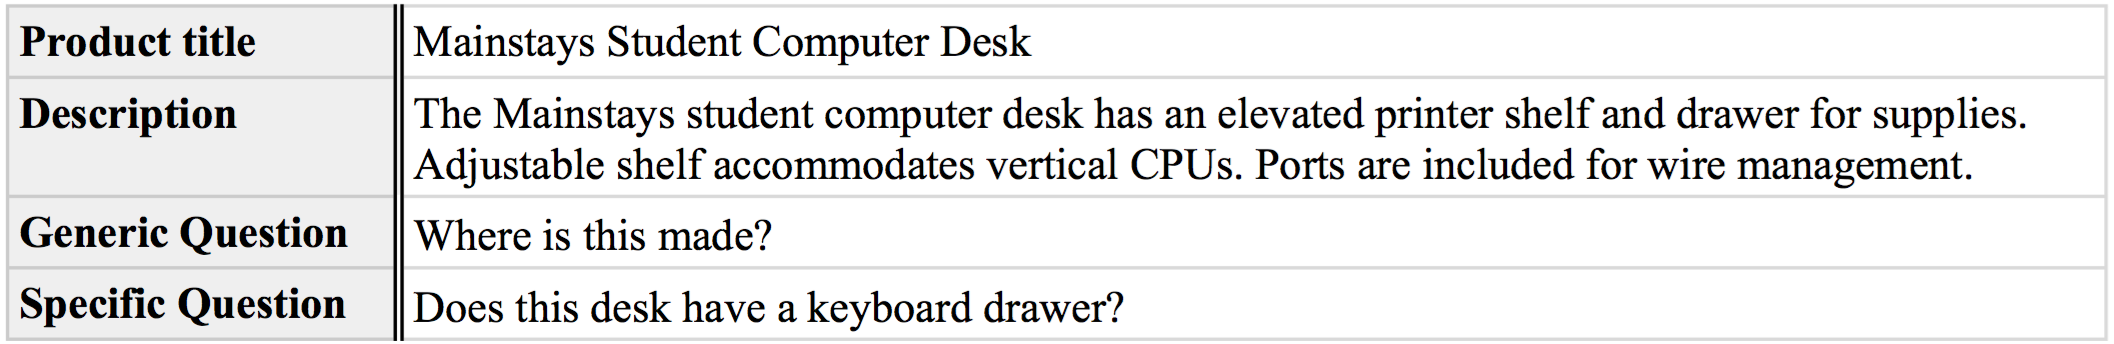
\includegraphics[width=\textwidth]{amaz-ex.png}
    \caption{Sample product description from amazon.com paired with a generic and a specific clarification question.}\label{amazon-ex-1}
\end{figure*}


\section{Model for Automatically Predicting Specificity Level}\label{classifier}

We annotate a set of 3000 questions from the Amazon dataset \cite{rao2019answer} with generic/specific labels using Amazon Mechanical Turk workers. Each question was annotated by three annotators and we take the majority as the label for that question.\footnote{In x\% of cases when there was no majority, we pick a label at random.} 
Given this annotated data, we want to train a machine learning model that can learn to predict the specificity level given a context and a question. We use some of the features described in Louis and Nenkova's work \cite{louis2011automatic} and introduce some new context-based features relevant to our setting. Based on these features, we train a logistic regression model to make a binary prediction (-1: generic, 1: specific) given a context and a question. We use the Support Vector Regression (SVR) model with Radial Basis Function (RBF) kernel. Gao et al. \shortcite{Gao2019PredictingAA}, in their work of analyzing language in social media post, claim SVR with RBF has the best performance in predicting text specificity.

%\begin{figure*}[h]
%\centering
%	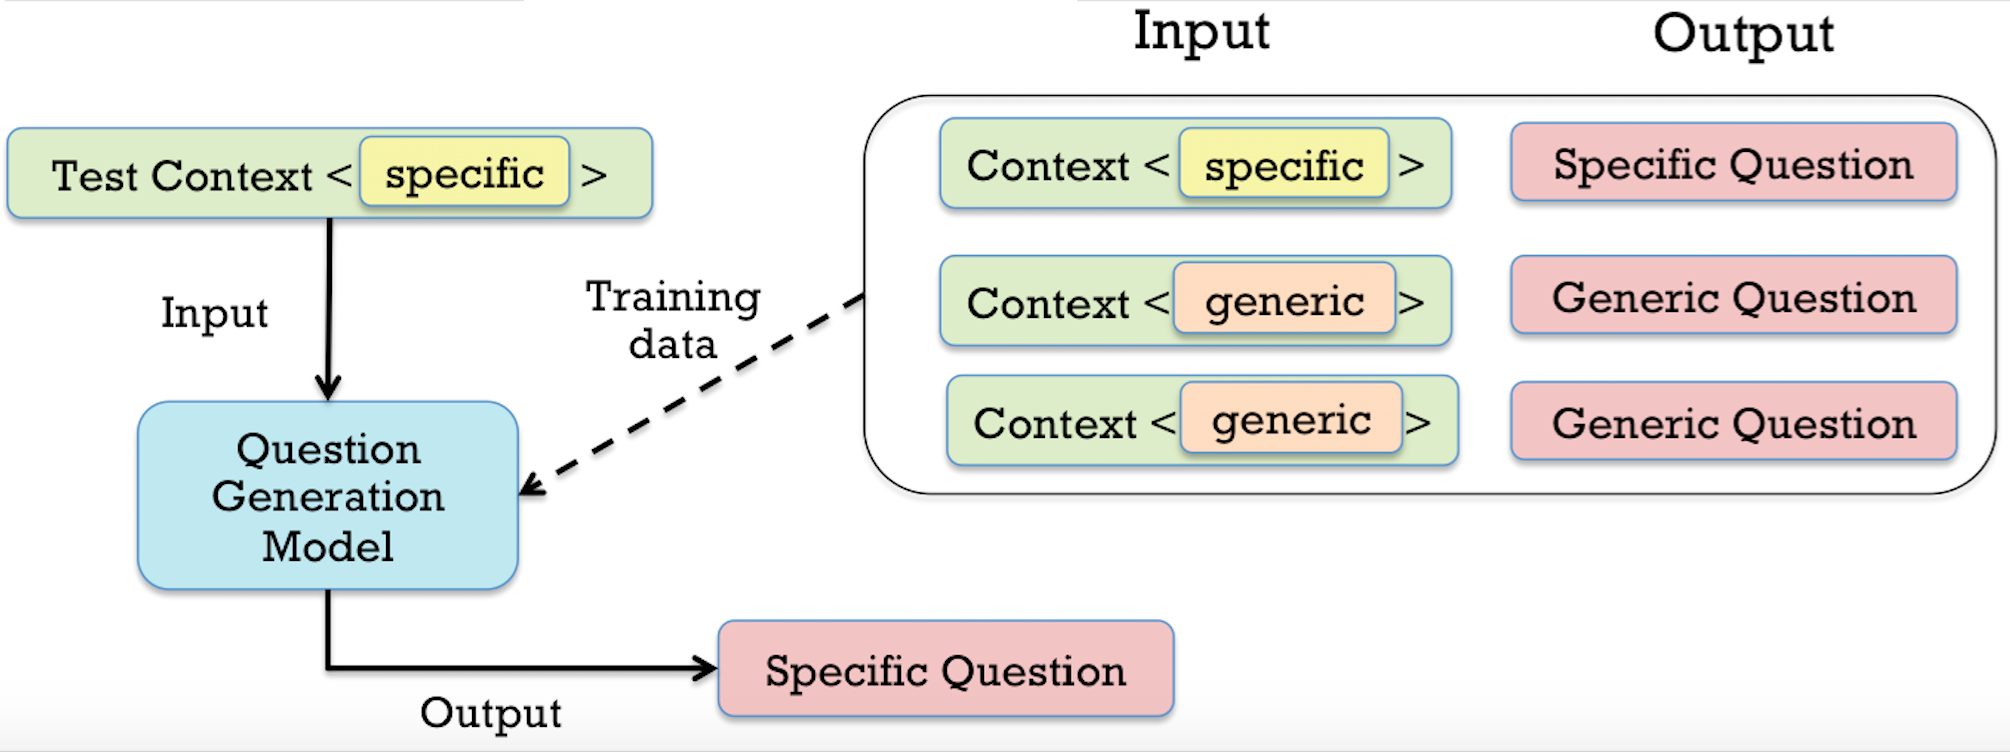
\includegraphics[scale = 0.3]{roadmap.png}
%    \caption{The behaviour of our model during test time.}\label{roadmap}
%\end{figure*}

\section{Specificity-Controlled Question Generation Model}\label{model}
The key idea behind sequence-to-sequence approaches is that given large amounts of input, output sequence pairs, the model learns internal representations such that at test time, given an input sequence, it generates the appropriate output sequence. 
We use the specificity classifier described in the previous section to label all the questions in the training (and tune) data with generic/specific labels. 
We use these labels to append each context with the \textit{$<$specific$>$} tag when the question paired with the context is labeled as specific and with the \textit{$<$generic$>$} tag when the question paired with the context is labeled as generic.
We train an attention-based sequence-to-sequence learning model \cite{luong2015effective} on (context+specificity, question) pairs using maximum likelihood objective. 
At test time, given a new context appended with the desired level of specificity, we generate a question at that level of specificity.


\section{Results and Conclusion}
We evaluate our model on the Amazon clarification questions dataset \cite{rao2019answer}. We find that our specificity classifier is able to predict the level of specificity of the question to the context with $76 \%$ accuracy. 
We also conduct preliminary experiments to evaluate our specificity-controlled question generation model. We use our classifier to annotate $\sim90,000$ questions from the Amazon dataset with their level of specificity and find that our question generation model trained on these (context+specificity, questions) pairs is able to generate questions at the desired level of specificity in most cases. We are in the process of evaluating our model outputs using human annotators. In this work, we thus introduce a semi-supervised approach to controlling the level of specificity of clarification questions to a given context.

% include your own bib file like this:
%\bibliographystyle{acl}
%\bibliography{coling2018}

\bibliography{specificity_controlled_clarification}
\bibliographystyle{acl}

\end{document}
